\documentclass[10pt,a4paper]{article}
	\usepackage[french]{babel}
	\usepackage[utf8]{inputenc}
	\usepackage[T1]{fontenc}

	\usepackage{amsmath}
	\usepackage{amsfonts}
	\usepackage{amssymb}
	
	\usepackage{calc}
	\usepackage{subcaption}
	\usepackage{graphicx}

	\usepackage{multicol}
		\setlength{\columnsep}{1cm}

	\usepackage{array}
		\newcolumntype{G}[1]{>{\raggedleft\arraybackslash}m{#1}}
		\newcolumntype{D}[1]{>{\raggedright\arraybackslash}m{#1}}
	\usepackage[squaren,Gray]{SIunits}

	\usepackage{xlop}
	\AtEndDocument{\label{lastpage}}
	
	\usepackage{geometry}
		\geometry{hmargin=2.5cm,vmargin=2.5cm}
	
		\usepackage{eso-pic}
		\newcommand{\HRule}{\rule{\linewidth}{0.5mm}}
		\newcommand{\blap}[1]{\vbox to 0pt{#1\vss}}
		\newcommand\AtUpperLeftCorner[3]{%
		 	\put(\LenToUnit{#1},\LenToUnit{\dimexpr\paperheight-#2}){\blap{#3}}%
		}
		\newcommand\AtUpperRightCorner[3]{%
		  	\put(\LenToUnit{\dimexpr\paperwidth-#1},\LenToUnit{\dimexpr\paperheight-#2}){\blap{\llap{#3}}}%
		}

	\usepackage{fancyhdr}
		\pagestyle{fancy}
		\fancyhfoffset{10pt}
		\lhead{\ecole}
		\chead{\matiere}
		\rhead{\Cusrus}
		\lfoot{\prof}	
		\cfoot{\me}
		\rfoot{\thepage/\pageref{lastpage}}
		\renewcommand{\headrulewidth}{0.4pt}
		\renewcommand{\footrulewidth}{0.4pt}
	 
	\usepackage{color}
		\definecolor{pblue}{rgb}{0.13,0.13,1}
		\definecolor{pgreen}{rgb}{0,0.5,0}
		\definecolor{pred}{rgb}{0.9,0,0}
		\definecolor{pgrey}{rgb}{0.46,0.45,0.48}
	
		\usepackage{xcolor}
		\definecolor{codegreen}{rgb}{0,0.6,0}
		\definecolor{codegray}{rgb}{0.5,0.5,0.5}
		\definecolor{codepurple}{rgb}{0.58,0,0.82}
		\definecolor{backcolour}{rgb}{0.95,0.95,0.92}
	
	\usepackage{listings}
		\lstdefinestyle{mystyle}{  
			    commentstyle=\color{codegreen},
			    keywordstyle=\color{magenta},
			    numberstyle=\tiny\color{codegray},
			    stringstyle=\color{codepurple},
			    basicstyle=\ttfamily\footnotesize,
			    breakatwhitespace=false,         
			    breaklines=true,                 
			    captionpos=b,                    
			    keepspaces=true,                 
			    numbers=left,                    
			    numbersep=5pt,                  
			    showspaces=false,                
			    showstringspaces=false,
			    showtabs=false,                  
			    tabsize=2
		}
		\lstset{style=mystyle}

		\setcounter{tocdepth}{3}

	\usepackage{hyperref}                 
		\hypersetup{
			hyperfigures = true,
			colorlinks = true,
			linkcolor=pblue
			}

%%%%%%%%%%%%%%%%%%%%%%%%%%%%%%%%%%%%%%%%%%%%%%%%%%%%%%%%%%%%%%%%%%%%%%%%%%%%%%%%%%%%%%%%%%%%%%%%
%
% 								Info Perso
%
%%%%%%%%%%%%%%%%%%%%%%%%%%%%%%%%%%%%%%%%%%%%%%%%%%%%%%%%%%%%%%%%%%%%%%%%%%%%%%%%%%%%%%%%%%%%%%%%

% Nom de l'élève			- \me
	\newcommand{\me}{Mathurin \textsc{Cartron}}
% Nom du reférent matière 	- \prof
	\newcommand{\prof}{Maxime \textsc{Maria}} 
% Matière 					- \matiere
	\newcommand{\matiere}{Moteur 3D}
% Cursusse 					- \Cusrus
	\newcommand{\Cusrus}{Master ISICG/CRYPTIS}
% Année dans ce Cursus 		- \Prog			
	\newcommand{\Prog}{Semestre 1}
% Numéros INE 				- \ine
	\newcommand{\ine}{}
% Nom de l'école 			- \ecole
	\newcommand{\ecole}{Université de limoges}
% Titre du document 		- \titre
	\newcommand{\titre}{Projet de \matiere}
% Sous titre du document 	- \soustitre
	\newcommand{\soustitre}{Compte Rendu}

\author{\me}
\title{\titre}
\date{\today}
\makeatletter

\begin{document}

%%%%%%%%%%%%%%%%%%%%%%%%%%%%%%%%%%%%%%%%%%%%%%%%%%%%%%%%%%%%%%%%%%%%%%%%%%%%%%%%%%%%%%%%%%%%%%%%
%
% 								   Page de garde
%
%%%%%%%%%%%%%%%%%%%%%%%%%%%%%%%%%%%%%%%%%%%%%%%%%%%%%%%%%%%%%%%%%%%%%%%%%%%%%%%%%%%%%%%%%%%%%%%%

	\begin{titlepage}
		\enlargethispage{2cm}
		\begin{center}
			\makebox[\textwidth]{
\includegraphics[width=0.3\paperwidth]{logo.jpg}}\\
			\vspace*{1cm}
			\HRule\\
				\vspace*{.5cm}
				\textsc{\LARGE{\titre}}\\
				\vspace*{.7cm}
				\Large{\soustitre}\\
				\vspace*{.2cm}
			\HRule
			\vspace*{.7cm}
			\begin{tabular}{D{7cm} G{7cm}}
				Élèves :  	&  Professeur : \\
				\me 		&  \prof  \\
			\end{tabular}
		\end{center}
		\vspace*{.7cm}
		\begin{multicols}{2}
			\tableofcontents
			\listoftables
			\listoffigures
			\lstlistoflistings
		\end{multicols}
		% \centering{\Cusrus -- \Prog \\}
		\vspace*{4cm}
	\end{titlepage}

\ClearShipoutPicture

%%%%%%%%%%%%%%%%%%%%%%%%%%%%%%%%%%%%%%%%%%%%%%%%%%%%%%%%%%%%%%%%%%%%%%%%%%%%%%%%%%%%%%%%%%%%%%%%
%
% 								   Content
%
%%%%%%%%%%%%%%%%%%%%%%%%%%%%%%%%%%%%%%%%%%%%%%%%%%%%%%%%%%%%%%%%%%%%%%%%%%%%%%%%%%%%%%%%%%%%%%%%

\section{Introduction}
	Le but de ce projet est de mettre en œuvre les différentes méthodes vues en cours et en TP, au travers d'une application de visualisation interactive de scènes 3D. L'objectif est d'implémenter des méthodes de rendu temps-réel pour réaliser des effets plus ou moins complexes. Parmi ces effets, on peut citer le light culling, le forward+, le calcul des ombres portées (shadow mapping, shadow volume), l'SSAO, l'FXAA et le bloom. Chacun de ces effets présente des défis spécifiques qui seront abordés dans le cadre de ce projet.

	\paragraph{Une longue absence} % (fold)
		En raison d'une longue absence dont vous connaissez la raison, j'ai pris un lourd retard dans mon travail. Par conséquent, je me contenterai de rendre le travail des TPs malgré les efforts que j'ai pu fournir pour le rattraper. Bien que cela ne couvre pas l'ensemble de ce qui était prévu pour ce projet, je suis conscient de l'importance de rendre quelque chose de complet et de bonne qualité. Je ferai de mon mieux pour atteindre cet objectif en privilégiant une bonne compréhension de notion qu'un projet entier mais baclé.
	% paragraph Une longue absence (end)

	\paragraph{Guacamole}
		Malheureusement, j'ai également été confronté à un autre obstacle qui a encore aggravé mon retard : la panne de "guacamole" durant les vacances de Noël. Cette panne m'a empêché de travailler pendant les vacances et a considérablement affecté ma progression. Malgré tout, j'ai fait de mon mieux pour rattraper mon retard à la rentrer, même si je ne parviens pas à couvrir tous les aspects prévus pour ce projet.
	% paragraph Guacamole (end)

	\paragraph{De l'aide de mes camarades}
		Heureusement, mes camarades m'ont apporté leur soutien et m'ont aidé à surmonter ces difficultés. Grâce à leur assistance, j'ai pu avancer dans mon travail et commencer à mettre en œuvre les différentes méthodes vues en cours et en TP. Cependant, je dois admettre que, malgré ma volonté de livrer un travail original et indépendant, il y a probablement plus de similarité entre le travail de mes camarades et le mien qu'il n'y en aurait eu sans leur intervention. En effet, ils ont dû déboguer mon code en se servant du leur, ce qui a inévitablement laissé des traces dans mon travail final. Je tiens à préciser que, malgré ces circonstances difficiles, j'ai fait de mon mieux pour assurer l'originalité de mon travail et éviter toute forme de plagiat. Si, malgré mes efforts, il y a des parties de mon travail qui présentent une forte similarité avec celui de mes camarades, je m'engage à le signaler explicitement dans les fichiers code et à préciser les contributions de chacun.
	% paragraph De l'aide de mes camarades (end)
	
\section{Contenu}

	\subsection{Architecture des TP}
		Au début du TP1, nous avons recu un projet qui allait évoluer jusqu'à la fin (TP6). L'objectif était de ne disposer que d'un seul projet Visual Studio, en utilisant un système de lab\_works pour gérer les différentes étapes du projet global.

		\paragraph{}Le lab\_works était organisé de manière à séparer les différents éléments du projet en plusieurs répertoires, chacun ayant un rôle précis :

		\begin{itemize}
			\item Le répertoire "src" contenait le code source du projet, organisé en plusieurs sous-répertoires selon leur fonction (par exemple, "core", "graphics", "input", etc.).
			\item Le répertoire "lib" contenait les bibliothèques externes utilisées par le projet (par exemple, "glew", "glfw", etc.).
			\item Le répertoire "data" contenait les données utilisées par le projet (par exemple, les modèles 3D, les textures, etc.).
		\end{itemize}

		\paragraph{}En utilisant cette architecture, nous avons pu travailler de manière organisée et efficace sur chaque TP, en ajoutant progressivement de nouvelles fonctionnalités au projet.

	\subsection{Le lab\_works\_manager} % (fold)
		En outre, le dossier lab\_works était divisé en sous-dossiers, un pour chaque TP. Ainsi, chaque TP disposait de son propre lab\_works, qui contenait tous les fichiers nécessaires pour compiler et exécuter le projet (shaders et le code du workspace).

		\paragraph{}Pour faciliter la navigation entre les différents lab\_works, nous avons mis en place un lab\_works\_manager. Ce dernier était accessible depuis le menu principal de l'application et permettait de passer d'un lab\_works à l'autre sans avoir à recompiler le code. Cette fonctionnalité a été particulièrement aprécier pour pouvoir comparrer nos différents TP entre eux et entre nous quelque soit l'avancement de chacun.

		\paragraph{Chargement d'un lab\_works} % (fold)
			Pour illustrer comment le lab\_works\_manager fonctionnait, je vais maintenant vous montrer le morceau de code qui permettait de charger un lab\_works. Dans la fonction \texttt{void LabWorkManager::drawMenu()} il suffisait de rajouter et de décliner pour chaque TP le code suivant:

			\lstinputlisting[language=C++ ,firstline=17, lastline=31,caption=Appel d'un lab\_works dans le lab\_works\_manager]{../m3d_isicg-main/src/lab_works/common/lab_work_manager.cpp}
			
		
		% paragraph Chargement d'un lab\_works (end)
	% subsection Le lab\_works manager (end)

	\subsection{Le lab\_works} % (fold)
		La classe LabWork1 est une classe dérivée de BaseLabWork et est utilisée pour implémenter le premier TP. Elle possède les méthodes suivantes :

		\begin{itemize}
			\item[\textbf{init()}] : méthode appelée au lancement de l'application pour initialiser les données de la scène et les données OpenGL.
			\item[\textbf{animate(float)}] : méthode appelée à chaque frame pour mettre à jour les données de la scène.
			\item[\textbf{render()}] : méthode appelée à chaque frame pour dessiner la scène à l'écran.
			\item[\textbf{handleEvents(SDL\_Event)}] : méthode appelée pour gérer les événements envoyés par SDL (par exemple, les entrées clavier ou souris).
			\item[\textbf{displayUI()}] : méthode appelée pour afficher l'interface utilisateur de la scène.
		\end{itemize}
		
		\paragraph{} % (fold)
			La classe LabWork1 possède également plusieurs membres privés qui stockent les données de la scène et les données OpenGL :
		% paragraph (end)
		
		\begin{itemize}
			\item[\textbf{\_triangle}] : un tableau de Vec2f qui contient les coordonnées du triangle à dessiner à l'écran.
			\item[\textbf{\_program}] : un identifiant OpenGL pour le programme de shaders utilisé pour dessiner la scène.
			\item[\textbf{\_vbo}] : un identifiant OpenGL pour le VBO (Vertex Buffer Object) utilisé pour stocker les données du triangle.
			\item[\textbf{\_vao}] : un identifiant OpenGL pour le VAO (Vertex Array Object) utilisé pour stocker les données de configuration de l'attribut de position du triangle.
			\item[\textbf{\_bgColor}] : une Vec4f qui contient la couleur de fond de l'application.
			\item[\textbf{\_shaderFolder}] : une chaîne de caractères qui contient le chemin vers le répertoire où se trouvent les shaders utilisés par cette classe.
		\end{itemize}
		
		\subsubsection{La méthode init()} % (fold)
			La méthode init() s'occupe d'initialiser toutes les données de la scène et de configurer OpenGL. Elle commence par appeler la méthode init() de la classe BaseLabWork, qui s'occupe de configurer SDL et OpenGL. Ensuite, elle charge et compile les shaders nécessaires pour dessiner la scène, crée le VAO et le VBO, et initialise les autres données de la scène.
		% subsubsection La méthode init() (end)

		\subsubsection{La méthode animate(float)} % (fold)
			La méthode animate(float) met à jour les données de la scène en fonction du temps écoulé depuis le dernier frame. Elle peut par exemple animer des objets en fonction de leur vitesse ou de leur accélération.
		% subsubsection La méthode animate(float) (end)

		\subsubsection{La méthode render()} % (fold)
			La méthode render() s'occupe de dessiner la scène à l'écran. Elle commence par nettoyer le framebuffer avec la couleur de fond (\_bgColor) et active le programme de shaders (\_program). Ensuite, elle active le VAO (\_vao) et appelle la fonction OpenGL glDrawArrays() pour dessiner le triangle stocké dans le VBO (\_vbo).
		% subsubsection La méthode render() (end)

		\subsubsection{La méthode handleEvents(SDL\_Event)} % (fold)
			La méthode handleEvents(SDL\_Event) est appelée à chaque frame pour gérer les événements envoyés par SDL. Elle peut par exemple gérer les entrées clavier ou souris pour permettre à l'utilisateur de naviguer dans la scène ou de changer les paramètres de l'application. Ce n'est pas utile dans le premier TP mais pas la suite je déplasserai la caméras avec. 
		% subsubsection La méthode handleEvents(SDL\_Event) (end)

		\subsubsection{La méthode displayUI()} % (fold)
		La méthode displayUI() s'occupe d'afficher l'interface utilisateur de la scène. Elle peut utiliser la bibliothèque de l'interface utilisateur (UI) de votre choix (par exemple, ImGui) pour afficher des éléments tels que des boutons, des sliders, etc. qui permettent à l'utilisateur de contrôler l'application.
		% subsubsection La méthode displayUI() (end)

	% subsection Le lab\\_works (end)

	\subsection{Présentation des 6 TPs} % (fold)
		Le fonctionnement de lab\_works et lab\_works\_manager restant quasiment le même jusqu'à la fin du TP6 (nous allons bien sur rajouter des chose dedans) Voici une description des 6 sujets de TP que nous avons abordés dans le cadre de ce projet. Ci dessous une image de synthèse de chacun d'entre eux. (\textit{cf} Figure \ref{fig:TPs})

		\begin{figure}[!ht]
			\centering
			\begin{subfigure}[b]{0.32\textwidth}
				\centering
				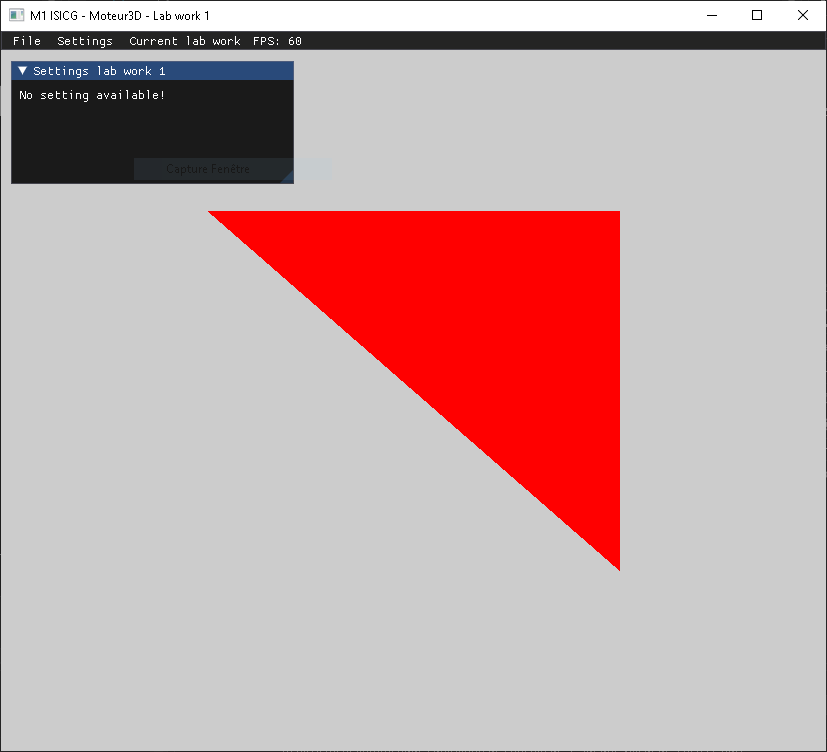
\includegraphics[width=.9\textwidth]{figures/TP1.png}
				\caption{TP1}\label{fig:TP1}
			\end{subfigure}
			\hfill
			\begin{subfigure}[b]{0.32\textwidth}
				\centering
				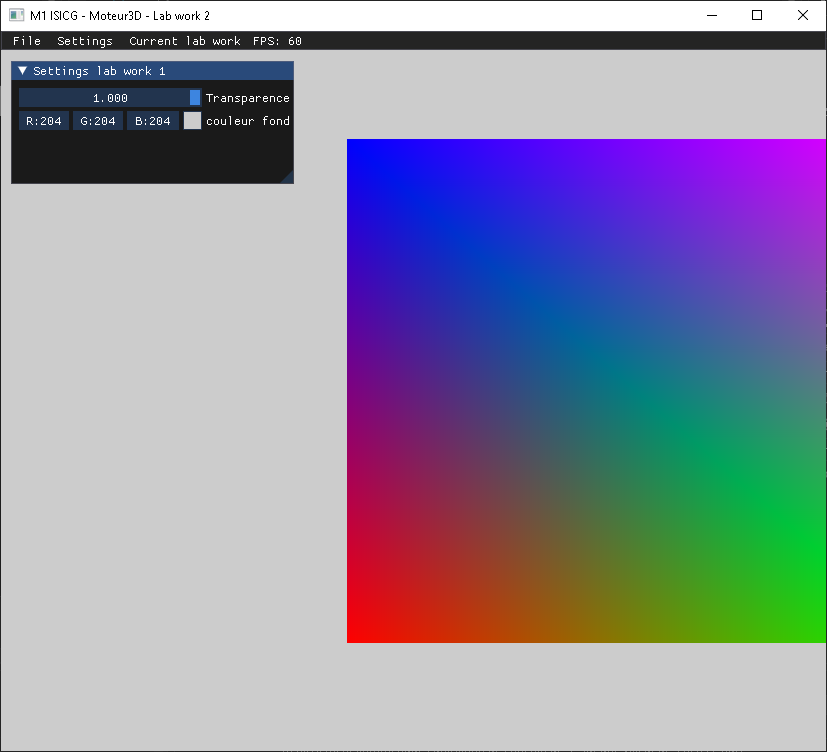
\includegraphics[width=.9\textwidth]{figures/TP2.png}
				\caption{TP2}\label{fig:TP2}
			\end{subfigure}
			\hfill
			\begin{subfigure}[b]{0.32\textwidth}
				\centering
				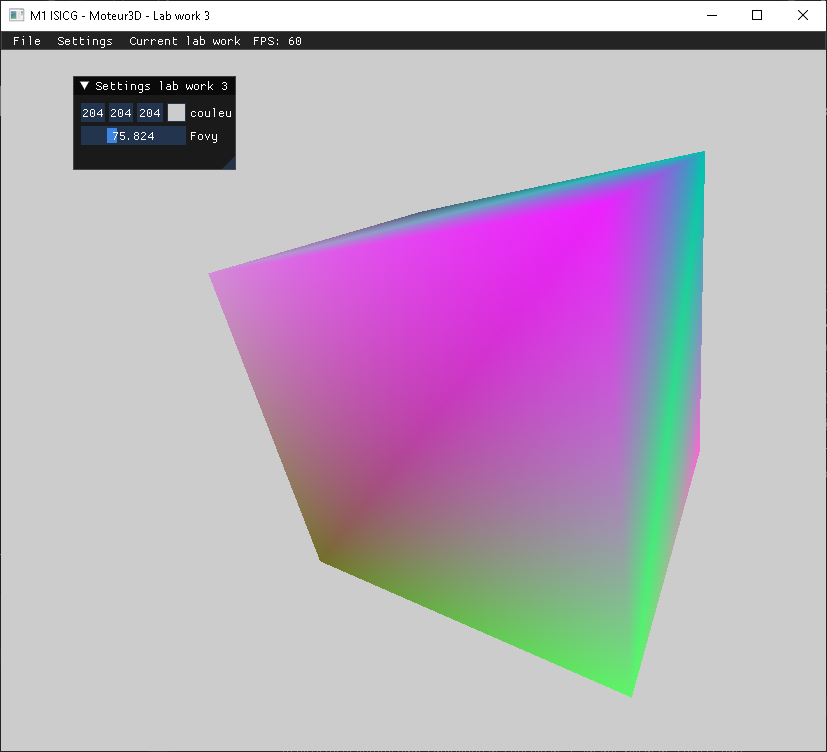
\includegraphics[width=.9\textwidth]{figures/TP3.png}
				\caption{TP3}\label{fig:TP3}
			\end{subfigure}
			\hfill
			\begin{subfigure}[b]{0.32\textwidth}
				\centering
				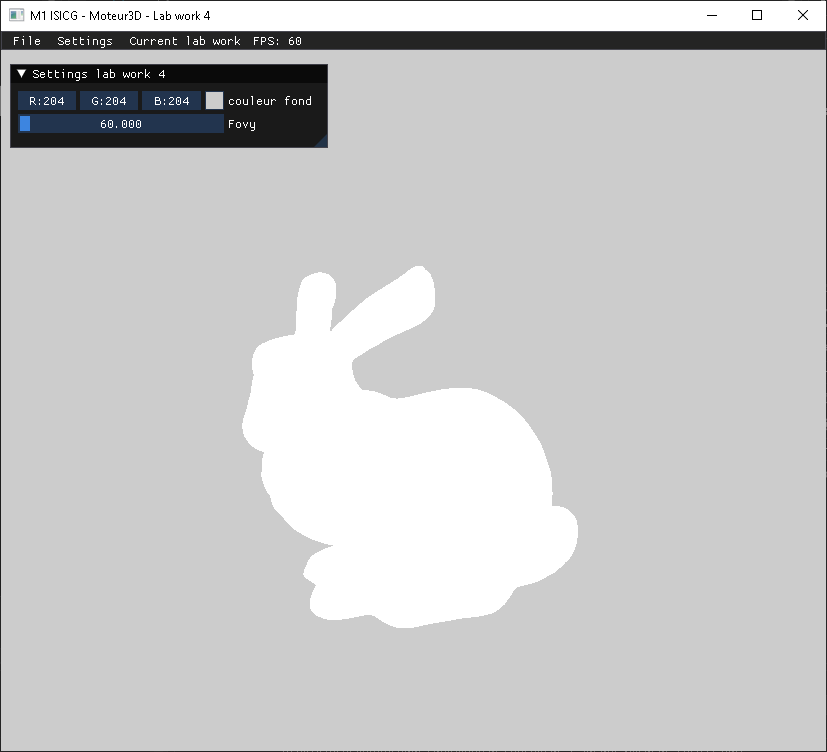
\includegraphics[width=.9\textwidth]{figures/TP4.png}
				\caption{TP4}\label{fig:TP4}
			\end{subfigure}
			\hfill
			\begin{subfigure}[b]{0.32\textwidth}
				\centering
				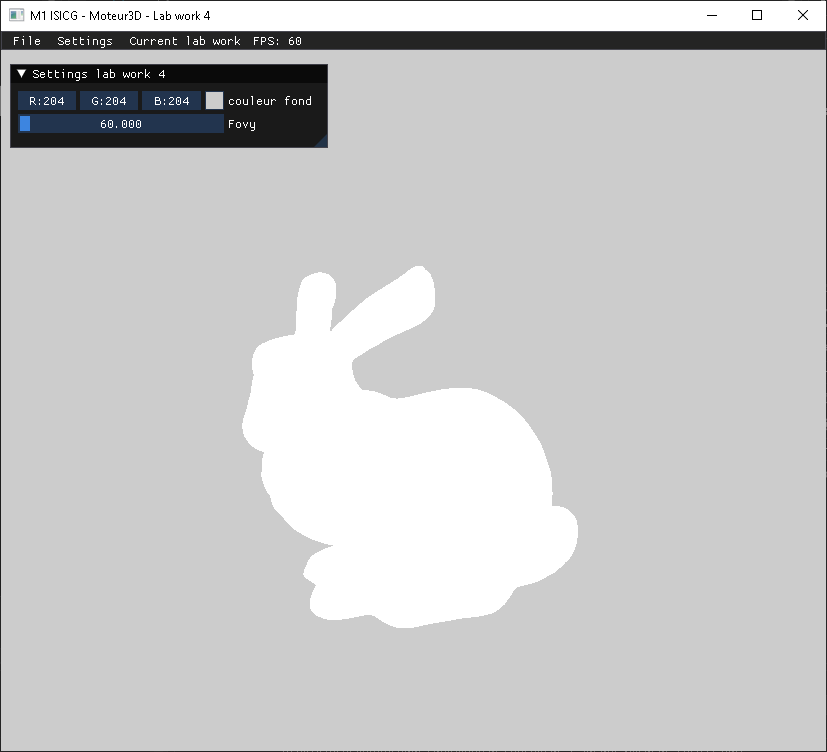
\includegraphics[width=.9\textwidth]{figures/TP5.png}
				\caption{TP5}\label{fig:TP5}
			\end{subfigure}
			\hfill
			\begin{subfigure}[b]{0.32\textwidth}
				\centering
				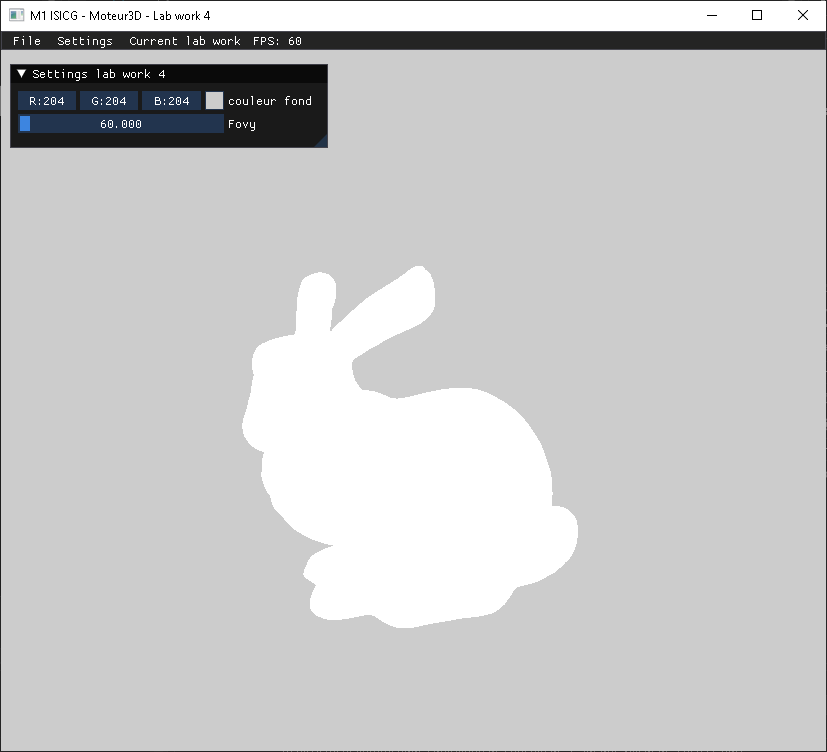
\includegraphics[width=.9\textwidth]{figures/TP6.png}
				\caption{TP6}\label{fig:TP6}
			\end{subfigure}
			\caption{Rendu de touts les TPs}\label{fig:TPs}
		\end{figure}

		\begin{itemize}
			\item\textbf{TP1} : L'objectif de ce TP était simplement d'afficher un triangle en 2D sur le plan image. Pour ce faire, nous avons dû apprendre à utiliser les fonctionnalités de base de OpenGL, telles que la création d'un programme de shaders, la gestion de VAO et de VBO, et l'utilisation de glDrawArrays().  (\textit{cf} Figure \ref{fig:TP1})
			\item\textbf{TP2} : Dans le TP2, nous avons affiché un quad en utilisant un VBO de type "Indexed" et en utilisant des shaders de couleur. Nous avons également animé le quad en le faisant se déplacer de gauche à droite et en modifiant son opacité.  (\textit{cf} Figure \ref{fig:TP2})
			\item\textbf{TP3} : Il a consisté à afficher un cube multicolore qui tournait sur lui-même en utilisant une caméra freefly. Nous avons appris à créer et à manipuler une matrice de vue pour contrôler la position et l'orientation de la caméra. (\textit{cf} Figure \ref{fig:TP3})
			\item\textbf{TP4} : Nous avons chargé un modèle 3D depuis un fichier (le bunny) et avons calculé l'éclairage local de se model. Nous avons aussi vue les éclairages plus avancer comme l'éclairage diffus et l'éclairage spéculaire du model de Phong. (\textit{cf} Figure \ref{fig:TP4})
			\item\textbf{TP5} : Il visait à manipuler des textures discrètes pour changer l'apparence de nos objets. Nous avons appris à charger et à appliquer des textures sur nos modèles 3D en utilisant des shaders de texture. (\textit{cf} Figure \ref{fig:TP5})
			\item\textbf{TP6} : Pour finir, le TP6 a consisté à mettre en place un pipeline de deferred rendering et à appliquer un post-traitement simple sur notre image. Nous avons appris à utiliser les techniques de deferred rendering pour séparer les différentes composantes de notre scène (couleur, position, normale, etc.) et à effectuer un rendu en plusieurs étapes pour obtenir une image finale de meilleure qualité. Nous avons également appris à utiliser les techniques de post-traitement pour améliorer l'apparence de notre image finale (par exemple, en utilisant l'effet de bloom). (\textit{cf} Figure \ref{fig:TP6})
		\end{itemize}

	% subsection Présentation de 6 TP (end)
	
	\subsection{TP1 : Manipulation des shaders} % (fold)
		Dans le cadre de ce projet, nous avons étudié l'utilisation des shaders avec OpenGL. Les shaders sont des programmes qui s'exécutent sur la carte graphique et qui permettent de définir comment les données de géométrie et de texture doivent être transformées et rendues à l'écran. Nous avons mis en place différents shaders au cours de ce projet, en utilisant le langage GLSL (OpenGL Shading Language), pour ajouter des effets tels que l'éclairage, les textures et les couleurs à nos scènes 3D. Nous avons appris à créer et à utiliser des shaders de vertex, de fragment et de geometry, ainsi qu'à passer des données aux shaders via les variables uniformes et les VBO. Pour le premier TP rien d'impossible : afficher un triangle rouge. 

		\subsubsection{Mise en place du fragment Shader et Vertex Shader} % (fold)
			La variable aVertexPosition est une variable d'entrée de type vec3 envoyée à l'emplacement 0 et contenant les coordonnées du vertex. La variable varSortieVS est une variable de sortie du shader de vertex qui sera envoyée au shader de fragment. Dans la fonction principale, la position du vertex est affectée à gl\_Position.
			
			\lstinputlisting[language=C++ ,caption=Vertex Shader du TP 1]{../m3d_isicg-main/src/lab_works/lab_work_1/shaders/lw1.vert}
			
			\paragraph{} % (fold)
				Le code suivant utilise la directive \#version 450 pour indiquer la version 4.5 du GLSL. La variable fragColor est déclarée comme une variable de sortie de type vec4 envoyée à l'emplacement de sortie 0. Dans la fonction principale, la valeur (1.0, 0.0, 0.0, 1.0) est affectée à fragColor, ce qui indique que chaque fragment sera affiché en rouge.
			% paragraph (end)
			
			\lstinputlisting[language=C++ ,caption=Fragment Shader du TP 1]{../m3d_isicg-main/src/lab_works/lab_work_1/shaders/lw1.frag}

		
		% subsubsection Mise en place du fragment Shader et Vertex Shader (end)

		\subsubsection{Le VAO et VBO} % (fold)
			Un Vertex Array Object (VAO) est un objet OpenGL qui stocke les informations de configuration des données de géométrie. Il permet de mémoriser les différentes configurations de VBO (Vertex Buffer Object, ou "tampon de sommets") et d'attributs de vertex, afin de pouvoir les rendre facilement. Par ailleur, un Vertex Buffer Object (VBO) est un tampon de mémoire qui stocke les données de géométrie (par exemple, les coordonnées des sommets, les couleurs, les normales, etc.). Il permet de transférer ces données de manière efficace vers le pipeline de rendu, sans avoir à les envoyer à chaque frame.

			\paragraph{}Le code ci-dessous crée un VAO et un VBO, puis configure l'attribut 0 du VAO pour utiliser les données du VBO. L'attribut 0 du VAO est activé et sa taille et son type sont définis. Le VBO et le VAO sont liés en indiquant la position de départ et l'espace entre chaque sommet dans le VBO. Enfin, l'attribut 0 du VAO est lié au descripteur d'attribut 0 du shader.

			\lstinputlisting[language=C++ ,firstline=110, lastline=112,caption=Création VBO TP1]{../m3d_isicg-main/src/lab_works/lab_work_1/lab_work_1.cpp}
			\lstinputlisting[language=C++ ,firstline=121, lastline=135,caption=Création VAO TP 1]{../m3d_isicg-main/src/lab_works/lab_work_1/lab_work_1.cpp}
		% subsubsection Le VAO et VBO (end)	
	% subsection TP1 Manipulation des shaders (end)

	\subsection{TP2 : On affiche un quad} % (fold)

		\subsubsection{L'EBO} % (fold)		
			Dans ce second TP j'ai créé ma première EBO. C'est un tampon de mémoire qui stocke les indices des sommets d'un maillage 3D. Il permet de réduire la quantité de données à envoyer au pipeline de rendu en ne transférant que les sommets nécessaires, au lieu de tous les sommets du maillage. Cela peut être particulièrement utile lorsque plusieurs objets partagent des sommets en commun, car cela permet d'éviter de les envoyer plusieurs fois. Pour utiliser un EBO, il suffit de le lier au VAO et de spécifier les indices des sommets à dessiner en utilisant une des fonctions de rendu d'OpenGL, comme glDrawElements().
			
			\lstinputlisting[language=C++ ,firstline=27, lastline=34,caption=Données qui serviront pour la création d'une EBO]{../m3d_isicg-main/src/lab_works/lab_work_2/lab_work_2.cpp}
		% subsubsection L'EBO (end)
		
		\subsubsection{Les varible uniforme} % (fold)
			Les variables uniformes sont des variables de shader qui ont la même valeur pour tous les sommets ou pixels d'une image. Elles permettent de passer des données du programme OpenGL vers les shaders de manière efficace, car elles ne nécessitent pas de stockage en mémoire pour chaque sommet ou pixel.
		
			\lstinputlisting[language=C++ ,firstline=127, lastline=128,caption=Création des variables Uniform dans le cpp du tP2]{../m3d_isicg-main/src/lab_works/lab_work_2/lab_work_2.cpp}

			\lstinputlisting[language=C++ ,firstline=214, lastline=221,caption=MàJ des variables Uniform dans le cpp du tP2]{../m3d_isicg-main/src/lab_works/lab_work_2/lab_work_2.cpp}

			\lstinputlisting[language=C++ ,firstline=3, lastline=11,caption=Utilisation des variables Uniform dans le Shader]{../m3d_isicg-main/src/lab_works/lab_work_2/shaders/lw2.vert}

		% subsubsection Les varible uniforme (end)
	
	% subsection TP2 :On affiche un quad (end)

	\subsection{TP3 Rotation du cube et caméra} % (fold)
		Dans le TP3, vous avez rencontré un problème lors de l'utilisation de la caméra, qui se manifestait par un comportement inattendu ou des erreurs lors du rendu de la scène 3D. Après investigation, j'ai découvert que le problème était causé par le fait que je n'avais pas correctement instancié la caméra avant de l'utiliser dans votre code.

		\subsubsection{Création du Cube} % (fold)
			La création d'un cube en 3D avec OpenGL peut être relativement simple, car il suffit de définir les positions de ses sommets et de les assembler en triangles pour former la géométrie de l'objet. Cependant, cette tâche peut être fastidieuse et prendre du temps, en particulier lorsque l'on utilise un tampon d'indices (EBO) pour spécifier les triangles.

			\lstinputlisting[language=C++ ,firstline=12, lastline=26,caption=Création d'un cube TP 3]{../m3d_isicg-main/src/lab_works/lab_work_3/lab_work_3.cpp}
		
		% subsubsection création du Cube (end)

		\subsubsection{La matrice MVP} % (fold)
			La matrice MVP (Model View Projection) est une matrice de transformation. Elle est composée de trois matrices : la matrice de modèle, la matrice de vue et la matrice de projection. Ces matrices permettent de définir la position, l'orientation et l'échelle de l'objet, ainsi que la position et l'orientation de la caméra et la manière de projeter l'objet sur l'écran. La matrice MVP est obtenue en multipliant ces trois matrices entre elles et est utilisée pour transformer les coordonnées des sommets de l'objet 3D dans le repère de l'écran.

			\lstinputlisting[language=C++ ,firstline=12, lastline=16,caption=Utilisation de la matrice MVP TP 3]{../m3d_isicg-main/src/lab_works/lab_work_3/shaders/lw3.vert}

			\paragraph{} % (fold)
				Dans mon code j'aurais trois foncitons qui mettrons à jours les inofrmations de ces matric pour les shaders en passant par des variable uniforme : \texttt{\_updateViewMatrix()}, \texttt{\_updateProjectionMatrix()} et \texttt{\_updateModelMatrix()}
			% paragraph (end) 

		% subsubsection La matrice MVP (end)
		
		\subsubsection{Ajout d'une caméra} % (fold)
			Une caméra Free Fly en OpenGL permet de déplacer et de faire pivoter la caméra dans l'espace 3D de manière libre. Elle est utilisée pour naviguer dans l'espace 3D, comme dans les jeux vidéo ou les logiciels de modélisation 3D. La position de la caméra est mise à jour en utilisant des matrices (le V et P de la matrice MVP).

			Il a fallu mettre à jour le code de la caméra pour qu'elle fonctionne. J'ai aussi eu un problème avec la caméra : après de longues heures de recherche, j'ai réalisé que le programme pouvait être compilé et exécuté sans jamais instancier la caméra (bien sûr, elle ne fonctionne pas). Cela m'a pris du temps avant de me rendre compte de l'erreur, car je pensais que mon code était correct alors qu'il était simplement incomplet.
		% subsubsection Ajout d'une caméra (end)

	% subsection TP3 Rotation du cube et caméra (end)
	
	\subsection{TP4 Le bunny et la lumière} % (fold)
		Pour afficher un modèle 3D dans ce TP, il était nécessaire de utiliser le code fourni dans le dossier "models" qui nous permettait de charger des maillages 3D. Nous avons dû éditer le fichier "triangle\_mesh.cpp" pour qu'il puisse charger et configurer les composants nécessaires pour l'affichage, tels que VAO, VBO et EBO.

		\subsubsection{La fin du code de Triangle\_mesh.cpp} % (fold)
			Voici le code qui permet de configurer les VBO et VAO pour utiliser un maillage de triangles avec OpenGL. Le VBO contient les données des sommets, comme leur position, leur normale, leur coordonnée de texture et leur tangente et bitangente. Le VAO stocke les informations sur la façon de lire ces données dans le VBO. Un EBO est également utilisé pour stocker les indices des sommets à dessiner, ce qui permet de ne pas avoir à répéter les données des sommets. La configuration des VAO et VBO est effectuée en spécifiant la position, le format et l'offset des différentes données dans le VBO et en les connectant au VAO. Les données des indices sont chargées dans l'EBO et liées au VAO.

			\lstinputlisting[language=C++ ,firstline=75, lastline=120,caption= Fonction \_setupGL TP4]{../m3d_isicg-main/src/lab_works/common/models/triangle_mesh.cpp}

			Pour ce qui concerne ce TP, il se peut que mon code soit très similaire à celui de Timothée car il m'a beaucoup aidé à comprendre comment gérer l'affichage 3D (VAO, VBO, EBO). Même si cela peut affecter ma note, je préfère le mentionner afin d'éviter tout problème de plagiat.
		% subsubsection La fin du code de Triangle\_mesh.cpp (end)

		\subsubsection{Une seule matrice MVP} % (fold)
			Pour ce TP, j'ai utilisé une seule matrice MVP pour transmettre les paramètres au shader, contrairement au TP précédent où j'en avais utilisé plusieurs. Pour mettre à jour la matrice MVP, j'ai multiplié la matrice de projection de la caméra, par la matrice de vue de la caméra, puis par la matrice de transformation de mon mesh. J'ai ensuite envoyé le résultat à mon programme de shader en utilisant la fonction \texttt{glProgramUniformMatrix4fv}.
			 
			\lstinputlisting[language=C++ ,firstline=172, lastline=175,caption= Matrice MVP TP4]{../m3d_isicg-main/src/lab_works/lab_work_4/lab_work_4.cpp}
		% subsubsection Un seul matrrice MVP (end)

		\subsubsection{Le shader} % (fold)
			Pour ce TP, j'ai dû ajouter de nombreux paramètres au shader pour prendre en compte l'éclairage selon le modèle de Phong. Cela a nécessité un code plus complexe pour le shader. Dans ce code, nous calculons l'éclairage de Phong en utilisant les paramètres d'entrée du vertex shader. Nous calculons la direction de la lumière et de la vue, ainsi que la normale du vertex. Ensuite, nous calculons la composante diffuse en utilisant la direction de la lumière et la normale, ainsi que la composante spéculaire en utilisant la réflection de la lumière sur la surface et la direction de la vue. Enfin, nous combinons ces composantes avec la couleur ambiante pour obtenir la couleur finale de fragment.


			\lstinputlisting[language=C++ ,firstline=17, lastline=37,caption= Matrice MVP TP4]{../m3d_isicg-main/src/lab_works/lab_work_4/shaders/mesh.frag}
		% subsubsection Le shader (end)

	% subsection TP4 Le bunny et la lumière (end)

	\subsection{Le TP5 une première scène} % (fold)
		Malheureusement, j'ai dû arrêter de travailler sur le TP5 avant d'avoir fini. Je n'ai pas eu le temps de rédiger l'intégralité du compte rendu, mais vous pouvez vous rendre compte de mon travail en examinant le code du programme et du Lab Work du TP5. Désolé pour cette inconvenience.
	
	% subsection Le TP5 une première scène (end)
\section{Conclusion}
	En conclusion, j'ai réalisé un grand nombre de tâches durant ce TP. J'ai commencé par afficher un triangle en 2D sur le plan image, puis j'ai affiché un quad multi-couleur animé avec une gestion de l'opacité. J'ai ensuite affiché un cube multicolore qui tournait sur lui-même avec une caméra Free Fly. J'ai chargé un modèle 3D depuis un fichier et j'ai calculé l'éclairage local selon le modèle de Phong. Malheureusement, je n'ai pas eu le temps de terminer les TPs et de rédiger un compte rendu complet, mais j'espère que vous avez pu découvrir les différentes tâches que j'ai réalisées grâce au lab Works.

%%%%%%%%%%%%%%%%%%%%%%%%%%%%%%%%%%%%%%%%%%%%%%%%%%%%%%%%%%%%%%%%%%%%%%%%%%%%%%%%%%%%%%%%%%%%%%%%
%
% 								   Exemple
%
%%%%%%%%%%%%%%%%%%%%%%%%%%%%%%%%%%%%%%%%%%%%%%%%%%%%%%%%%%%%%%%%%%%%%%%%%%%%%%%%%%%%%%%%%%%%%%%%

		%%%%%%%%%%%%%%%%%%%%% TABLE

		% \begin{table}[!ht]
		% 	\centering
		% 	\begin{tabular}{|*{9}{c|}}
		% 		\multicolumn{9}{c}{RGB2HSV}\\								
		% 		\hline
		% 		block					& 8x8		& 16x16		& 32x32	 	& 	64x64	& 128x128	& 256x256	& 512x512	& 1024x1024 \\
		% 		\hline
		% 		temps nvproof (us)		& 118,72	& 71,808	& 76,515 	& 	x		& x			& x			& x			& x \\
		% 		temps chronoGPU (us)	& 125,76	& 77,856	& 84,416 	& 	x		& x			& x			& x			& x \\
		% 		\hline
		% 		\multicolumn{9}{c}{HSV2RGB 1D} \\
		% 		\hline
		% 		block					& 8x1		& 6x1		& 32x1		& 64x1		& 128x1		& 256x1		& 512x1		& 1024x1 \\
		% 		\hline
		% 		temps nvproof (us)		& 325,28	& 174,85	& 99,328	& 69,494	& 70,206	& 73,355	& 78,725	& 84,589 \\
		% 		temps chronoGPU (us)	& 332,256	& 179,952	& 110,624	& 75,36		& 81,312	& 82,672	& 84,512	& 96,288 \\
		% 		\hline
		% 	\end{tabular}
		% 	\caption{Comparatif de temps }\label{tab:temps}
		% \end{table}

		%%%%%%%%%%%%%%%%%%%%% SUBFIGURE
				
		% \begin{figure}[!ht]
		% 	\centering
		% 	\begin{subfigure}[b]{0.32\textwidth}
		% 		\centering
		% 		\includegraphics[width=.9\textwidth]{../screens/serie_0_3_20_600_600.png}
		% 		\caption{Aléatoire}\label{fig:1}
		% 	\end{subfigure}
		% 	\hfill
		% 	\begin{subfigure}[b]{0.32\textwidth}
		% 		\centering
		% 		\includegraphics[width=.9\textwidth]{../screens/serie_1_3_20_600_600.png}
		% 		\caption{Permutation aléatoire}\label{fig:2}
		% 	\end{subfigure}
		% 	\hfill
		% 	\begin{subfigure}[b]{0.32\textwidth}
		% 		\centering
		%  		\includegraphics[width=.9\textwidth]{}
		% 		\caption{Coupe optimale}\label{fig:3}
		% 	\end{subfigure}
		% 	\caption{Comparaison des différents algorithmes}\label{fig:rendu}
		% \end{figure}


\end{document}
